\documentclass[12pt, oneside]{book}

\usepackage{graphicx}  % this is for includegraphics
\graphicspath{{figures/}}

\usepackage{setspace}
\onehalfspacing % this sets spacing to 1.5 

\usepackage{subfig}
\usepackage{amsmath}
\usepackage{amsthm} % for theorems, lemmas etc
\usepackage{amsfonts}
\usepackage{lipsum} % to generate the lipsum random text in the sample
\usepackage{tikz}
\usepackage{siunitx}
\usetikzlibrary{calc,decorations.pathmorphing,patterns}


\usepackage[colorlinks=true, urlcolor=blue, pdfborder={0 0 0}]{hyperref}
\hypersetup{
     colorlinks   = true,
     citecolor    = blue
}

\theoremstyle{plain}
\newtheorem{theorem}{Theorem}[section]
\newtheorem{proposition}[theorem]{Proposition}
\newtheorem{lemma}[theorem]{Lemma}
\newtheorem{corollary}[theorem]{Corollary}
\newtheorem{fact}[theorem]{Fact}

\theoremstyle{definition}
\newtheorem{definition}[theorem]{Definition}
\newtheorem{example}[theorem]{Example}
\newtheorem{remark}[theorem]{Remark}
\newtheorem{remarks}[theorem]{Remarks}

\newcommand{\Cov}{\mathrm{Cov}}
\newcommand{\Var}{\mathrm{Var}}

\begin{document}

\begin{titlepage}
\begin{center}
        \vspace{-2cm}
Mathematical Finance MSc Dissertation MTH775P, 2018/19 
		\\
        \Huge
        \textbf{Accelerated Grids}
        \\        
        \vspace{0.4cm}
        \LARGE
        Optimizing Solvers for Financial Partial Differential Equations
        \\        
        \vspace{0.4cm}        
        \textbf{Mustafa Berke Erdis, ID 180883925}% student name and number        
        \\
        \large Supervisor: Dr. Sebastian del Bano Rollin
        \\
        \vspace{0.9cm}
        
\includegraphics[scale=0.23]{QMCrest.png}
        \\
        \vspace{0.9cm}        
        \LARGE 
        A thesis presented for the degree of\\
        Master in Sciences in \emph{Mathematical Finance}\\
        \vspace{0.7cm}        
        \Large
        School of Mathematical Sciences\\ 
        and \emph{School of Economics and Finance}\\
        Queen Mary University of London \\
    \end{center}
\end{titlepage}


\chapter*{Declaration of original work}
\begin{flushright}
This declaration is made on \today.
\end{flushright}


{\bf Student's Declaration:}
I, Mustafa Berke Erdis, hereby declare that the work in this thesis 
is my original work. I have not copied from any other students' work, work of 
mine submitted elsewhere,  or from any other sources except where due reference or acknowledgement is made explicitly in the text, nor has any part been written for me by another person.

Referenced text has been flagged by:
\begin{enumerate}
\item Using italic fonts, {\bf and} % LaTeX: {\it text}  
\item using quotation marks ``\ldots '', {\bf and}
\item explicitly mentioning the source in the text.
\end{enumerate}

%This excludes any definitions known from your modules or undethat can be found in an undergraduate text book.

\newpage

\thispagestyle{empty}
        \begin{flushright}
                This work is dedicated to my family.
        \end{flushright}
\vspace{\stretch{2}}\null



\chapter*{Acknowledgements}
Here you thank people that have helped you in the journey. \\
\lipsum[100] % replace this by your text

\chapter*{Abstract}
\begin{center}
\small 
Here you write a short summary, around 10 lines, of your work. \\
\lipsum[100]% replace this by your text
\end{center}       


\begin{flushright}
Queen Mary University of London\\
12${}^{\text{th}}$ August 2019
\end{flushright}

\tableofcontents

\chapter{Introduction}
In Ancient Greece, Thales was scorned for his poverty. Later that year, Thales utilized his skills in astrology to forecast an increase in olive yields. Using his limited capital, he rented oil presses in winter. Months later, over the oil making season, many people rushed to the presses because of the high yields that Thales predicted. As he rented the presses over the winter, he forced the terms he pleased. Thales showed it was easy for philosophers to be rich if they chose it and practically used the first  financial derivative product \cite{thalesians}. 

In the modern world, financial derivatives are contracts between two or more parties. The value of the contract depends on one or several underlying assets. Commonly the assets are currencies, equities, bonds, interest rates, market indices or commodities. The vanilla call option gives the right but not the obligation to buy the underlying asset at the expiry date at a previously agreed strike price. Essentially, Thales bought call options for oil presses.  If the olive yields didn't come as Thales expected he didn't have the obligation to use the olive presses.  On the other hand, the vanilla put option gives the right but not the obligation to sell the underlying asset at the expiry date at a previously agreed strike price. Practical applications of the options include hedging or speculating the future asset price. Hence, accurately pricing the options is crucial for an efficient and mature financial market.

Merton and Scholes received the 1997 Nobel Prize in Economic Science for this work \cite{merton}. 

\section{Motivation of the Project}
Derivative pricing in the real world is a computationally intensive task. The existing numerical methods for partial differential equations are all constrained by the computational complexity. Being fast when evaluating new information is critical for the operations of hedge funds and investment banks. Therefore optimizing the existing numerical methods with hardware and software that can be installed on a trading floor is crucial. Goal of the project is to provide efficient methods for pricing options.

Purpose of this project to optimize numerical solutions of parabolic PDEs by testing high performance computing techniques and comparing compilers/os/32bit/64bit.
The idea of this project is to study how to take advantage of this parallelism and explore how much faster we can make these calculations.


Included in your ‘Introduction’ section should be a clear summary of  what  you  have  achieved  in  the  project  work  presented,  such  as  any  new  results, generalisations, corollaries, examples, new connections, or computer investigations.  The thesis is organized as follows.  Chapter 2 presents an introduction to financial derivatives, Black-Scholes model and finite difference models.  Chapter3 extends the 2d and gives examples of two dimensional heat equation.  Chapter 4 develops the numerical methods and techniques considered to solve the PDE-based models for the option pricing problems.  In the same chapter,  finite difference method with improved algorithms to solve a large tridiagonal systems is discussed.  Chapter 5 shows the numerical results of our numerical methods with several examples of.  Chapter 6 concludes the thesis.

\chapter{Pricing Financial Derivatives}\label{Pricing Financial Derivatives}
\section{The Risk Neutral Approach}
The Black-Scholes framework is a theoretical valuation formula for options. It reveals the relationship between the prices of the options and the underlying assets. Since almost all corporate liabilities can be viewed as combinations of options, the formula is applicable to common stocks and corporate bonds \cite{BS}. The Black-Scholes model makes the following assumptions:
\begin{itemize}
\item There does not exist any arbitrage opportunity in the financial market.  The traders can’t make instantaneous profit without any risk.
\item The underlying asset value follows a geometric Brownian Motion $dS = \mu S dt + \sigma S dB $ where $\mu$ denotes the average rate of growth of the underlying assets, $\sigma$ denotes the volatility of the asset price and B is a Brownian Motion.
\item The market is frictionless.  This means there are no transaction fees, the interest rates for borrowing and lending money from and to the bank are the same, every party  in  market  has  immediate  information  and  all  entities  are  available  at  anytime and in any size.
\end{itemize}

\subsection{Black-Scholes Partial Differential Equation}
The original model is used to price the vanilla  option, which is the simplest type of option. The dividends can be included in the Black-Scholes formula. Presence of dividends can be included in the Black-Scholes formula. Since it doesn't effect the performance, for the sake of simplicity we will assume there are no dividends paid. Under the assumptions of Black-Scholes framework, the call or put option price satisfies the parabolic partial differential equation.

\begin{equation}
\frac{\partial V}{\partial t} = rS\frac{\partial V}{\partial S}+\frac{1}{2} \sigma^2 S^2 \frac{\partial^2 V}{\partial S^2} - rV
\end{equation}

Framework shows the  price V(t,S)  of  a  European  option  driven  by  one underlying asset that satisfies the PDE where $r$, $\sigma$, $t$, $S$respectively denotes the risk-free interest rate, volatility, time and the underlying price.  It is assumed that $r$ and $\sigma$ are constants. In more complicated models such as stochastic volatility models they can be a function.We will consider the  PDE and conditions for the call options.  In order to price a vanilla call option the PDE needs to satisfy the following boundary and initial conditions. 

\begin{eqnarray}
C(0,t) &=& 0, \hspace{4pt} C(S_{\max},t)=S_{\max} - K e^{-r(T-t)}, \hspace{10pt} 0 \leq t \leq T \\[10pt]
C(S,T) &=& \max(S-K,0), \hspace{10pt} 0 \leq S \leq S_{\max}
\end{eqnarray}

\subsection{Derivation of the Black-Scholes Equation}
Black-Scholes model takes advantage of the properties of the geometric Brownian motion and It\^{o}'s lemma. 

\begin{definition} Brownian Motion \\
Brownian motion (also known as Wiener Process) was discovered by botanist Robert Brown as he observed a chaotic motion of particles suspended in water \cite{BM}. A  Brownian  motion, $B(t)$,  is  a  continuous-time  stochastic  process  with  the  following properties: 
\begin{itemize}
\item $ B(0) = 0 $.
\item $ B(t) $ is a continuous function of t.
\item For $ 0  \leq s < t $ the increment $ B(t) -  B(s)  $ has normal distribution  $ \mathcal{N}(0, t-s) $.
\item  For $ t_0  \leq  t_1 \leq ... \leq  t_n $ the increments $ B(t_k) - B(t_{k-1}) $ where $k=1, .... ,n $ are independent random variables.
\end{itemize}    
Brownian motion is the basic building block in stochastic calculus and geometric Brownian motion is used to model the stock prices in Black-Scholes model.
\end{definition}

\begin{lemma} It\^{o}'s Lemma:
Let $B(t)$ be a Brownian motion and $X(t)$ be an Ito process which satisfies the stochastic differential equation:
\begin{equation}
dX(t) = \mu(X(t),t)dt + \sigma(X(t),t)dB(t)
\end{equation} 
If $f(x, t)$ is twice continuously differentiable function then $f(X(t),t)$ is also an Ito drift-diffusion process \cite{klebaner}, with its differential given by:
\begin{equation}
d(f(X(t),t)) = \frac{\partial f}{\partial t}(X(t),t)dt + f'(X(t),t)dX + \frac{1}{2}f''(X(t),t)dX(t)^2
\end{equation} 
With $dX(t)^2$ given by: $dt^2 = 0$, $dt dB(t) = 0$ and $dB(t)^2 = dt$.
\end{lemma}

\begin{theorem}
Assume that the asset price $S$ follows a geometric Brownian motion.  Under the assumptions of Black-Scholes framework, the call or put option price $V(t,S)$ satisfies the parabolic partial differential equation
\begin{equation}
\frac{\partial V}{\partial t} = rS\frac{\partial V}{\partial S}+\frac{1}{2} \sigma^2 S^2 \frac{\partial^2 V}{\partial S^2} - rV
\end{equation}
\end{theorem}

\begin{proof}
Suppose an investor sets up a self-financing portfolio,  $ X(t)$, comprising one option and an $\Delta$ amount of the underlying asset. Therefore, value of the portfolio at time t is $X(t) = V(t) + \Delta S(t)$. 
Since the self-financing trading strategy has no capital influx or consumption, the value of portfolio change can be written as 
\begin{equation}
dX = dV + \Delta dS
\end{equation}

Applying the It\^{o}'s Lemma to the option price V(t,S)
\begin{equation}
dV = \frac{\partial V}{\partial t} dt + \frac{\partial V}{\partial S} (S,t) dS + \frac{1}{2}\frac{\partial^2 V}{\partial S^2}(S,t)dS^2
\end{equation}

Since the Black-Scholes model assumes that the stock price under the "market probability measure" follows a gBM. 
\begin{equation}
dS = \mu S dt + \sigma S dW
\end{equation}

Putting (1.4) and (1.6) together yields
\begin{equation}
dV = (\frac{\partial V}{\partial t} + \mu S \frac{\partial V}{\partial S} + \frac{1}{2} \sigma^2 S^2 \frac{\partial^2 V}{\partial S^2} + \Delta \mu S) dt + (\sigma S \frac{\partial V}{\partial S}+\Delta \sigma S) dW
\end{equation}

The fact that portfolio is risk-free implies that the second term involving the Brownian Motion, $dW$, must be zero.  This technique is known as delta-hedging , otherwise, we would have an arbitrage opportunity. Thus, $ \Delta = - \frac{\partial V}{\partial S}$.  Hence, the growth rate of the portfolio must be the risk free rate which can be summarized as $ dX = r X dt $. Substituting $\Delta$ and $dX$ yields

\begin{equation}
\frac{\partial V}{\partial t} + \frac{1}{2} \sigma^2 S^2 \frac{\partial^2 V}{\partial S^2} = r(V-S\frac{\partial V}{\partial S})
\end{equation}

Rearranging the equation to get famous Black-Scholes equation:
\begin{equation}
\frac{\partial V}{\partial t} = rS\frac{\partial V}{\partial S}+\frac{1}{2} \sigma^2 S^2 \frac{\partial^2 V}{\partial S^2} - rV
\end{equation}
\end{proof} 

\begin{definition}\label{bsAnal} The resulting partial differential equation can be solved analytically using the following boundary conditions and initial conditions for call options.
\begin{eqnarray}
\frac{\partial C}{\partial t} &=& rS\frac{\partial C}{\partial S}+\frac{1}{2} \sigma^2 S^2 \frac{\partial^2 C}{\partial S^2} - rC \\[10pt]
C(0,t) &=& 0, \hspace{4pt} C(S_{\max},t)=S_{\max} - K e^{-r(T-t)}, \hspace{10pt} 0 \leq t \leq T \\[10pt]
C(S,T) &=& \max(S-K,0), \hspace{10pt} 0 \leq S \leq S_{\max}
\end{eqnarray}

Solving the equations, the formulae \cite{wilmott} for European call is
\begin{eqnarray}
C = S \Phi (d_1) - K e^{-r(T-t)} \Phi (d_2) \\[10pt]
d_1 = \frac{log(S/K) + (r + \sigma^2/2)(T - t)}{\sigma \sqrt{T-t}} \\[10pt]
d_2 = d_1 - \sigma \sqrt{T-t}
\end{eqnarray}

The following parameters will be used for the research purposes of this project.
\begin{table}[h!]
\centering
 \begin{tabular}{||c c||} 
 \hline
 Parameter & Value\\ [0.5ex]
 \hline\hline
 Strike Price ($K$) & 1.0\\ 
 Volatility ($\sigma$) & 20 \% \\
 Risk Free Rate ($r$) & 5 \% \\
 Time to Expiry ($T$) & 2.0\\
 Maximum Share Price ($S_{max}$) & 2.0\\ [1ex] 
 \hline
 \end{tabular}
\end{table}
\end{definition}

\begin{definition} 
Black-Scholes PDE has coefficient that depend on $S$. Meaning that PDE is not space homogeneous. Log spot Black-Scholes PDE is an economically intrinsic way of looking at numbers, if two assets are similar it is conventional to investigate using the $x = ln S$ conversion. 

Applying the chain rule to the first and second order derivatives
\begin{equation}
\frac{\partial C}{\partial S} = \frac{\partial C}{\partial x} \frac{\partial x}{\partial S} = \frac{\partial C}{\partial x} \frac{1}{S}
\end{equation}
\begin{eqnarray}
\frac{\partial^2 C}{\partial S^2} = \frac{\partial }{\partial S} (\frac{\partial C}{\partial S}) = \frac{\partial }{\partial S} (\frac{\partial C}{\partial x} \frac{1}{S}) = -\frac{1}{S^2} \frac{\partial C}{\partial x} + \frac{\partial }{\partial S} \frac{\partial C}{\partial x} \frac{1}{S} = \\
 = -\frac{1}{S^2} \frac{\partial C}{\partial x} + \frac{\partial^2 C}{\partial x^2} \frac{1}{S^2} 
\end{eqnarray}

Substituting the transformed derivatives into the original PDE 
\begin{equation}
\frac{\partial C}{\partial t} = (r - \frac{\sigma^2}{2})\frac{\partial C}{\partial x}+\frac{1}{2} \sigma^2 \frac{\partial^2 C}{\partial x^2} - rC
\end{equation}

The transformation creates a PDE with constant coefficients rather than coefficients that depend on S. 

\end{definition}
\begin{remark}Untradable Assets\\ Modern financial engineering created derivatives using untradable assets as an underlying such as multi asset derivatives like equity baskets, weather derivatives, non-deliverable swaps and non-deliverable forwards. Non-deliverable forwards are for offshore investors that want to trade non-convertible currencies such as Brazilian Real, South Korean Won.  The Black-Scholes model is still used in these cases \cite{weather} \cite{basket} but not entirely applicable to assets that cannot be hedged.
\end{remark}


\section{Partial Differential Equations}
Since the foundation of the world humanity tried to understand and model the nature. Differential equations serves this purpose by enabling us to describe natural phenomena for instance, heat, sound and fluid flow. Differential equations can be classified in to two categories. Ordinary differential equations serve to model a movement space or plane, an example would be the trajectory of a projectile launched from a cannon follows a curve determined by an ordinary differential equation that is derived from Newton's second law.

On the other hand, partial differential equations modelles a function, a typical example is the heat distribution. This distinction usually makes PDEs much harder to determine an analytical solution than ordinary differential equations.  Therefore, we need to achieve a numerical solution to the problem. One of the most commong numerical method for partial differential equations is the finite difference methods. The methods consist of finding approximate solutions to the problem at a discrete set of points, normally on a rectangular grid of points. Finite difference methods are simple to construct and analyse but can compromise performance because of increased computational complexity when there are high dimensions. 

Feynman-Kac theorem \cite{klebaner}, establishes a link between partial differential equations and stochastic processes by writing the solution as a conditional expectation. Thanks to the theorem, Monte Carlo method is also utilized to find the numerical solutions to the partial differential equations. The convergence rate of Monte Carlo method for $n$ simulations can be denoted as $\mathcal{O}(n^{\frac{-1}{2}}) $ which holds for all dimensions ($d$).
The error in $d$ dimensional trapezoidal rule for twice continuously differentiable integrands is $\mathcal{O}(n^{\frac{-2}{d}}) $ \cite{glasserman}. Thus, Monte Carlo is a method of choice when evaluating higher dimensions.

\subsection{Heat Equation}
The heat equation is fundamental to financial engineering. Heat equation is a component in the Black-Schole equation and Black-Scholes equation can be transformed to the heat equation by changing variables \cite{capinski}. Therefore, understanding heat equation is crucial to grasping concepts of partial differential equations. Heat equation will serve as a benchmark with the following initial and boundary conditions.

\begin{eqnarray} \label{HeatBase}
u_t(x,t) &=& u_{xx}(x, t) \\[10pt]
u(0, t) &=& u(x_{max}, t) = 0, \hspace{10pt} 0 \leq t \leq T \\[10pt]
u(x, 0) &=& sin(\pi x), \hspace{10pt} 0 \leq x \leq x_{\max}
\end{eqnarray}

In our calculations, we will test the case where $T = 0.06$ and $x_{max} = 1.0$.

\begin{definition}\label{heatAnal} Analytical Solution of Heat Equation

Certain kinds of partial differential equations allows us to find an analytical solution with the help of the Separation of Variables technique.

\begin{eqnarray}
u(x,t) = X(x) T(t) \\[10pt]
u_{xx}(x, t) = X^{''}(x) T(t) \\[10pt]
u_t (x,t) = X(t) T^{'}(t)
\end{eqnarray}

Using the partial derivatives the equation $ u_t = u_{xx} $ becomes
\begin{equation}
\frac{T^{'}(t)}{T(t)}  = \frac{X^{''}(x)}{X(x)}
\end{equation}

Right hand side only depends on $x$ and the left hand side depends only on $t$. Therefore, the equation is valid only when each side is equal to a constant, which we set to $ \lambda $. Rearranging terms gives us the following equations:

\begin{equation}
\frac{T^{'}(t)}{T(t)}  = \frac{X^{''}(x)}{X(x)} = -\lambda \\[10pt]
\end{equation}
\begin{equation}\label{xlambda}
X^{''}(x)  + \lambda X(x) = 0 
\end{equation}
\begin{equation}\label{tlambda}
T^{'}(t) + \lambda T(t) = 0
\end{equation}

\begin{equation}
X(0) = X(1) = 0
\end{equation}

Solving for X(x) is an example case of Sturm-Liouville problem \cite{sepvar} with three cases. 
\begin{itemize}
\item Let $\lambda < 0$ and $\lambda = -k^2$. Then the solution to \ref{xlambda} is
$$ X = Ae^{kx} + Be^{-kx} $$
Using the boundary conditions yield $X(0) = A + B = 0 $ and $X(1) = Ae^{k} + Be^{-k} = 0$. Solving the equations $A=B=u=0$ which is a trivial solution, thus discarded.
\item Let $\lambda = 0$, the solution to \ref{xlambda} is
$$ X(x) = Ax + B $$
The boundary conditions imply $X(0) = B = 0$ and $X(1) = A= 0$. Thus this case is  discarded too.
\item Finally, let $\lambda>0$,the solution to \ref{xlambda} is
$$ X(x) = Acos(\sqrt{\lambda}x) + Bsin(\sqrt{\lambda}x) $$

The boundary conditions leads to $
X(0) = A = 0$ and $ X(1) = Bsin(\sqrt{\lambda}) = 0 $
Since we do not want a trivial solution where $B = 0$, the equation reduces to 
\begin{equation}
sin(\sqrt{\lambda}) = 0
\end{equation} 
Thus $ \sqrt{\lambda} = n \pi $ for $n = 1,2,3, ...$. 
Solution to \ref{xlambda} becomes,
\begin{equation}
X_n = b_n sin(n \pi x), \hspace{10pt} n=1,2,3, ...
\end{equation}
\end{itemize}

As we determined $ \lambda = n^2 \pi^2 $ for $n = 1,2,3, ...$.  Solving \ref{tlambda} for $T(t)$ gives the solution
\begin{eqnarray}
T^{'}(t) = -n^2 \pi^2 T(t)
T_n = c_n exp(-n^2 \pi ^2 t) \\[10pt]
\end{eqnarray}
where $c_n$'s are integration constants.

Putting the solution of $T(t)$ and $X(x)$ together,
\begin{equation}
u(x,t) = \sum_{n=1}^{\infty} B_n exp(-n^2 \pi ^2 t) sin(n \pi x)
\end{equation}
where we have set $B_n = c_n b_n$. The initial condition gives
\begin{equation} \label{initB}
u(x,0) = sin(\pi x) = \sum_{n=1}^{\infty} B_n sin(n \pi x)
\end{equation}
which is a Fourier sine series.  Solving for the $B_n$’s, we use the orthogonality property for the eigenfunctions $sin(n \pi x)$ 
    \[ \int_{0}^{1} sin(m \pi x) sin(\pi n x) dx = \begin{cases} \mbox{0,} & \mbox{if } m \neq n \\ \mbox{1/2,} & \mbox{m = n} \end{cases} = 0.5 \delta _{mn} \]
    
where $ \delta _{mn}$ is the kronecker delta,  
\[  \delta _{mn} = \begin{cases} \mbox{0,} & \mbox{if } m \neq n \\ \mbox{1,} & \mbox{m = n} \end{cases} \]

Solving \ref{initB} for $B_n$, multiplying both sides with $sin(m \pi x)$ and integrate from $0$ to $1$ and from the definition of kronecker delta yields
\begin{equation}    
B_n = 2 \int_{0}^{1} sin(\pi x) sin(\pi n x) dx = \frac{2sin(\pi n)}{\pi - \pi n^2}
\end{equation}
Combining the solutions
\begin{equation}
u(x,t) = \sum_{n=1}^{\infty} \frac{2sin(\pi n)}{\pi - \pi n^2} exp(-n^2 \pi ^2 t) sin(n \pi x)= exp(-\pi^2 t) sin(\pi x) 
\end{equation}
\end{definition}

\subsection{Two Dimensional Heat Equation}
The natural extension of our study of the one-dimensional problem would now be to investigate partial differential equations with more than one space-like dimension. When more than one space dimensions are involved, we have to deal with equations such as two dimensional heat equation or multi-asset black-scholes equation.  We will consider the following PDE and conditions for the purposes of research.

\begin{equation}
\frac{\partial u}{\partial t} = \frac{\partial^2 u}{\partial x^2} +\frac{\partial^2 u}{\partial y^2}
\end{equation}$  $
Initial and boundary condition
\begin{eqnarray} \label{HeatTwoBase}
u(x,y,0) = 1, \hspace{10pt} 0 \leq x \leq x_{\max}, \hspace{10pt} 0 \leq y \leq y_{\max} \\[10pt]
u(x, 0, t) = u(x, y_{max}, t) = 0, \hspace{10pt} 0 \leq t \leq T \\[10pt]
u(x, 0, t) = u(x, 1, t) = 0 , \hspace{10pt} 0 \leq t \leq T
\end{eqnarray}
In the calculations, we will test the case where $T = 0.06$, $x_{max} = 1.0$ and $y_{max} = 1.0$.

\begin{definition}\label{heat2Anal} Analytical Solution of Two Dimensional Heat Equation
Similarly, applying separation of variables method to the equation
\begin{eqnarray}
u(x,t) = X(x) Y(y) T(t) \\[10pt]
X^{''}(x) - B X(x) = 0 \\[10pt]
Y^{''}(y) - C (y) = 0 \\[10pt]
T^{'}(t) - (B + C) T(t) = 0 \\[10pt]
X(0) = X(1) = 0, \hspace{10pt} Y(0) = Y(1) = 0
\end{eqnarray}

In \ref{heatAnal}, we have already seen that the solutions to X(x) and Y(y) are
\begin{eqnarray} 
X_m (x) =  b_n sin(m \pi x) \\
Y_n (x) =  a_m sin(n \pi y)
\end{eqnarray}

Using these values to solve for $T(t)$ gives
\begin{equation}
T_{mn}(t) = c_{mn} exp(- \pi^2 (m^2 + n^2)t)
\end{equation}

Substituting the solutions yields
\begin{equation}
u_{mn}(x, y, t) = X_m(x) Y_n(y) T_{mn}(t)
\end{equation}
\begin{equation}
u(x, y, t) = \sum_{m=1}^{\infty} \sum_{n=1}^{\infty} A_{mn}  sin(m \pi x) sin(n \pi y) exp(- \pi^2 (m^2 + n^2)t)
\end{equation}
where $A_{mn} = b_n a_m c_{mn}$.
The initial condition gives
\begin{equation}
u(x, y, 0) = 1 = \sum_{m=1}^{\infty} \sum_{n=1}^{\infty}  A_{mn} sin(m \pi x) sin(n \pi y)
\end{equation}
which is a double Fourier sine series. Thus, the coefficient $A_{mn}$ is chosen such that
\begin{equation}
 A_{mn} = 4 \int_{0}^{1}  \int_{0}^{1} sin(\pi m x)  sin(\pi n y) dx dy = \frac{4(cos(\pi n) - 1)(cos(\pi m) - 1)}{\pi^2 m n} 
\end{equation}
Combining the solutions
\begin{multline}
u_{mn}(x, y, t) =  \sum_{m=1}^{\infty} \sum_{n=1}^{\infty} \frac{4(cos(\pi n) - 1)(cos(\pi m) - 1)}{\pi^2 m n}  \\ sin(m \pi x) sin(n \pi y)     exp(- \pi^2 (m^2 + n^2)t)
\end{multline}

\end{definition}



\section{Finite Difference Methods}
\subsection{Discretization}
Essentially, solving a PDE is the problem of finding a function which depends on values at infinitely many points. Naturally, the finite difference methods first step is to make the problem discrete that we are able to solve \cite{jwthomas}. As a result, we need to discretise the space dimensions and time dimension. The discretization procedure begins by replacing the domain $[0, x_{max}]$ x  $[0, T]$  by a set of mesh points. In order to get a $n$ x $m$ equally spaced mesh points the step sizes are calculated as $ \Delta t = \frac{T}{m}$, $\Delta x = \frac{x_{max}}{n}$.

\begin{figure}[!htb]
    \centering
        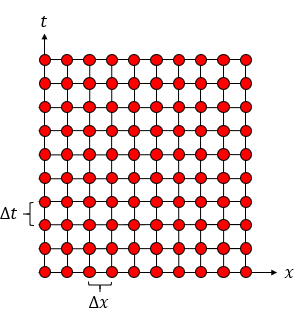
\includegraphics[scale=0.8]{Discretize.png}
    \caption{10 x 10 grid.}
\end{figure}
In order to replace our PDE, we need to utilize finite difference approximations for the partial derivatives. Notationally, we will define $u^n_i$ to be a function defined at the point $(i \Delta x, n \Delta t) $.

\begin{itemize}
        \item Forward difference: $ \frac{\partial u}{\partial t} = \frac{u^{n+1}_i - u^n_i}{\Delta t} + \mathcal{O}( \Delta t) $
        \item Central difference: $ \frac{\partial u}{\partial x} = \frac{u^n_{i+1} - u^n_{i-1}}{\Delta t}   + \mathcal{O}( \Delta x) $
        \item Backwards difference: $ \frac{\partial u}{\partial x} = \frac{u^{n}_i - u^n_{i - 1}}{\Delta t}  + \mathcal{O}( \Delta x) $
        \item Second order central difference: $ \frac{\partial^2 u}{\partial x^2} = \frac{u^n_{i+1}- 2u^n_i + u^n_{i-1}}{(\Delta x)^2}  + \mathcal{O}( \Delta x^2) $
\end{itemize}

We now have a grid that approximates our domain. Aiming to obtain a unique solution using numerical methods, we need initial and boundary conditions. Final step is applying the values given by such conditions.

\begin{figure}[!htb]
  \begin{minipage}[b]{0.5\textwidth}
    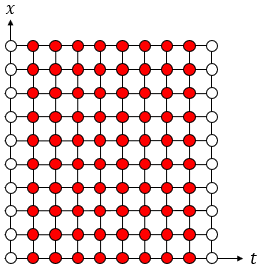
\includegraphics[width=\textwidth]{Boundary.png}
    \caption{Boundary conditions.}
  \end{minipage}
  \begin{minipage}[b]{0.5\textwidth}
    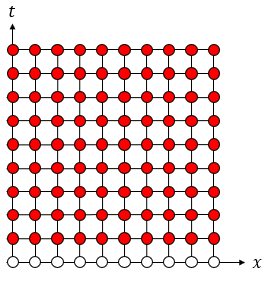
\includegraphics[width=\textwidth]{Initial.png}
    \caption{Initial condition.}
  \end{minipage}
\end{figure}

\subsection{Explicit Method}
Explicit method generalises the parabolic partial differential equation by applying the forward difference to the time derivative and the centred second difference (FTCS scheme).
\begin{equation} \label{gen}
 u_t = a(t, x)  u_{xx} + b(t, x) u_x + c(t, x) u
\end{equation}

We will be applying the finite differences to the equation  \ref{gen}  for the purposes of simplicity since heat equation and Black-Scholes equation can be generalized in the form for certain choices of coefficients. Applying the forward time and centred space differences where $ r = \frac{\Delta t}{\Delta x^2} $.

\begin{multline}
\frac{u^{n+1}_i - u^n_i}{\Delta t} = a(t, x)  \frac{u^n_{i+1}- 2u^n_i + u^n_{i-1}}{(\Delta x)^2}  + b(t, x)  \frac{u^{n}_{i+1} - u^{n}_{i-1}}{\Delta x} +   + c(t, x) u^n_i \\
u^{n+1}_i = u^n_{i + 1} (\frac{-r b(t,x)}{\Delta x} - r a(t, x)) + u^n_{i}(1 + 2 r a(t, x) - c(t, x) \Delta t) \\
+ u^n_{i - 1} (-r a(t, x) + \frac{r b(t, x)}{\Delta x})
\end{multline}

We will replace the coefficients of $ u^n_{i + 1},  u^n_i,  u^n_{i - 1}$  terms with $\gamma,  \alpha, \beta$ respectively. The formula reduces to

\begin{equation}
u_j^{n+1} = \gamma u_{j+1}^{n} + \beta u_{j}^{n} + \alpha u_{j-1}^{n} .
\end{equation}

The formula expresses one unknown nodal value directly in terms of known nodal values  \cite{evans}. It can be expanded as
\begin{multline}
u_1^{n+1} = \gamma u_{2}^{n} + \beta u_{1}^{n} + \alpha u_{0}^{n} \\
u_2^{n+1} = \gamma u_{3}^{n} + \beta u_{2}^{n} + \alpha u_{1}^{n} \\
.\\
\hspace{75pt} .\\
\hspace{150pt} .\\
u_{j-1}^{n+1} = \gamma u_{j}^{n} + \beta u_{j-1}^{n} + \alpha u_{j-2}^{n} 
\end{multline}

Using the boundary conditions and  initial condition, the expanded formula can be condensed in the following matrix form. 
$$
\begin{bmatrix} 
u_{1}^{n + 1} \\ 
u_{2}^{n + 1} \\ 
u_{3}^{n + 1} \\ 
.\\ 
.\\ 
.\\ 
u_{j - 1}^{n + 1}\\ 
\end{bmatrix} = \begin{bmatrix}
\alpha u_{0}^{n} \\ 
0 \\ 
0 \\ 
.\\ 
.\\ 
.\\ 
\gamma u_{j}^{n} \\ 
\end{bmatrix}  + \begin{bmatrix}  
\beta & \gamma & 0 & . & . & 0 \\ 
\alpha & \beta & \gamma & 0 & ... & . \\ 
0 & \alpha & \beta & \gamma & 0 & . \\ 
. & . & .  & . & . & . \\ 
. & . & .  & . & . & . \\ 
. & . & .  & . & . & \gamma \\ 
0 & 0 & 0 & 0 & \alpha & \beta \\ 
\end{bmatrix} \begin{bmatrix}  
u_{1}^{n} \\ 
u_{2}^{n} \\ 
u_{3}^{n} \\ 
.\\ 
.\\ 
.\\ 
u_{j - 1}^{n} \\ 
\end{bmatrix} 
$$

Deriving the coefficients   $\gamma,  \alpha, \beta$ in the case of heat equation yields
\begin{equation}
\alpha =  r \hspace{15pt} \beta = 1 - 2r \hspace{15pt} \gamma = r
\end{equation}

In the case of Black-Scholes formula, since the share price $S_j$ increases linearly with $\Delta x$ we can replace it as $S_j = j \Delta x$. 
\begin{equation}
\alpha =  \frac{\sigma^2 j^2 \Delta t}{2} - \frac{r j \Delta t}{2} \hspace{15pt} 
\beta = 1 - \sigma^2 j^2 \Delta t - r \Delta t \hspace{15pt} 
\gamma = \frac{\sigma^2 j^2 \Delta t}{2} + \frac{r j \Delta t}{2}
\end{equation}

Lastly, solving heat equation and Black-Scholes differs in time stepping. Black-Scholes formula is solved backwards in time. On the other hand, heat equation is solved forwards in time. 

\begin{figure}[!htb]
  \begin{minipage}[b]{0.5\textwidth}
    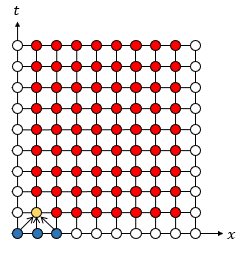
\includegraphics[width=\textwidth]{ExplicitHeat.png}
    \caption{Computational stencil \\of heat equation.}
  \end{minipage}
  \begin{minipage}[b]{0.5\textwidth}
    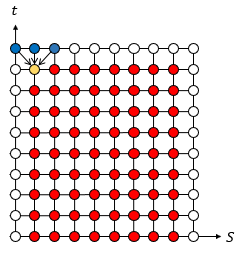
\includegraphics[width=\textwidth]{ExplicitBS.png}
    \caption{Computational stencil \\of Black-Scholes.}
  \end{minipage}
\end{figure}

\begin{figure}[!htb]
  \begin{minipage}[b]{0.5\textwidth}
    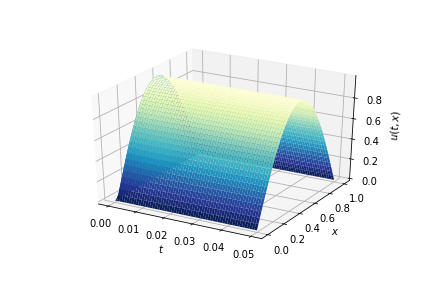
\includegraphics[width=\textwidth]{HeatExplicitGrid.png}
    \caption{Output grid of heat equation.}
  \end{minipage}
  \begin{minipage}[b]{0.5\textwidth}
    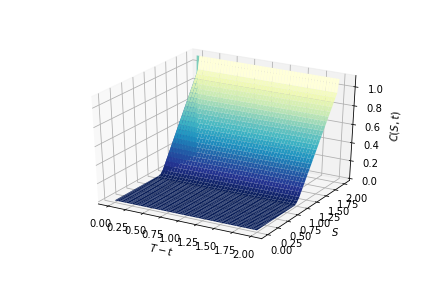
\includegraphics[width=\textwidth]{BSExplicitGrid.png}
    \caption{Output grid of Black-Scholes equation.}
  \end{minipage}
\end{figure}

\subsection{Crank-Nicholson Method}
The explicit method is computationally cheap. However, this brings a serious drawback, for explicit method to attain reasonable accuracy the step size must be kept small \cite{gdsmith}. Thankfully, the Crank-Nicolson finite difference scheme was introduced by John Crank and Phyllis Nicolson \cite{cn}. Considering numerous articles and publications in the financial engineering literature use Crank-Nicolson as the de-facto scheme for time discretisation, the method has become one of the most popular finite difference schemes for approximating the solution of the Black - Scholes equation and its generalisations \cite{tavella}.

 If we apply backwards time difference instead of forward time difference that Explicit method used and a central space approximation in space again, we get the BTCS scheme. Applying the BTCS to the base equation \ref{gen}. yields
    \begin{equation}
\frac{u^{n+1}_i - u^n_i}{\Delta t}  = a(t, x)  \frac{u^{n+1}_{i+1}- 2u^{n+1}_i + u^{n+1}_{i-1}}{(\Delta x)^2}  + b(t, x)  \frac{u^{n+1}_i - u^{n+1}_i}{\Delta t}  + c(t, x)  u^{n+1}_i
\end{equation}

Crank-Nicolson method takes a weighted average of the FTCS and BTCS schemes. Therefore the approximations become
$$ u(t,x) \approx \frac{1}{2} ( u^{n+1}_i +  u^n_i) $$
$$ \frac{\partial u}{\partial t} \approx \frac{u^{n+1}_i - u^n_i}{\Delta t} $$
$$ \frac{\partial u}{\partial x} \approx \frac{u^n_{i+1} - u^n_{i-1} + u^{n+1}_{i+1} - u^{n+1}_{i-1}}{4\Delta x} $$
$$ \frac{\partial^2 u}{\partial x^2} \approx \frac{u^n_{i+1}- 2u^n_i + u^n_{i-1} + u^{n+1}_{i+1}- 2u^{n+1}_i + u^{n+1}_{i-1}}{2(\Delta x)^2} $$

Applying the new finite differences to the base partial differential equation equation \ref{gen}
\begin{multline}
 (-A -B) u^{n+1}_{i+1} + (1 + 2A - C) u^{n+1}_i + (-A + B) u^{n+1}_{i-1} =  \\
=  (A+B) u^{n}_{i+1} + (1 - 2A + C) u^{n}_i + (A - B) u^{n}_{i-1}
\end{multline}
$$ A = a(t,x) \frac{\Delta t}{\Delta x^2},  B = b(t,x) \frac{\Delta t}{4\Delta x}, C = c(t,x) \frac{\Delta t}{2}$$ 

Note that in contrast to the FTCS scheme, we now have three unknowns in this equation, the three values of $u$ at the higher time level.  We respectively denote the coefficients in the right hand side as $\gamma, \beta, \alpha$ and coefficients in the left hand side as $\lambda, \theta, \omega$ for simplicity.
\begin{equation}
\lambda u^{n+1}_{i+1} + \theta u^{n+1}_i + \omega u^{n+1}_{i-1} =  \\
=  \gamma u^{n}_{i+1} + \beta u^{n}_i + \alpha u^{n}_{i-1}
\end{equation}

The left hand side groups the unknowns and the right hand side groups knowns. The system of equations can be  reduced to a matrix system. 

$$
\begin{bmatrix}  
\theta & \lambda & 0 & . & . & 0 \\ 
\omega & \theta & \lambda & 0 & ... & . \\ 
0 & \omega & \theta & \lambda & 0 & . \\ 
. & . & .  & . & . & . \\ 
. & . & .  & . & . & . \\ 
. & . & .  & . & . & \lambda \\ 
0 & 0 & 0 & 0 & \omega & \theta \\ 
\end{bmatrix}  \begin{bmatrix} 
u_{1}^{n + 1} \\ 
u_{2}^{n + 1} \\ 
u_{3}^{n + 1} \\ 
.\\ 
.\\ 
.\\ 
u_{j - 1}^{n + 1}\\ 
\end{bmatrix}= \begin{bmatrix}
\alpha u_{0}^{n} \\ 
0 \\ 
0 \\ 
.\\ 
.\\ 
.\\ 
\gamma u_{j}^{n} \\ 
\end{bmatrix}  + \begin{bmatrix}  
\beta & \gamma & 0 & . & . & 0 \\ 
\alpha & \beta & \gamma & 0 & ... & . \\ 
0 & \alpha & \beta & \gamma & 0 & . \\ 
. & . & .  & . & . & . \\ 
. & . & .  & . & . & . \\ 
. & . & .  & . & . & \gamma \\ 
0 & 0 & 0 & 0 & \alpha & \beta \\ 
\end{bmatrix} \begin{bmatrix}  
u_{1}^{n} \\ 
u_{2}^{n} \\ 
u_{3}^{n} \\ 
.\\ 
.\\ 
.\\ 
u_{j - 1}^{n} \\ 
\end{bmatrix}
$$

The problem reduces to a tridiagonal matrix system. This system of equations can be solved by various algorithms such as Gaussian elimination or Thomas algorithm.

\begin{figure}[!htb]
  \begin{minipage}[b]{0.5\textwidth}
    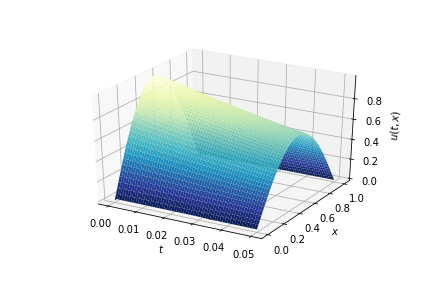
\includegraphics[width=\textwidth]{HeatCNGrid.png}
    \caption{Output grid of heat equation.}
  \end{minipage}
  \begin{minipage}[b]{0.5\textwidth}
    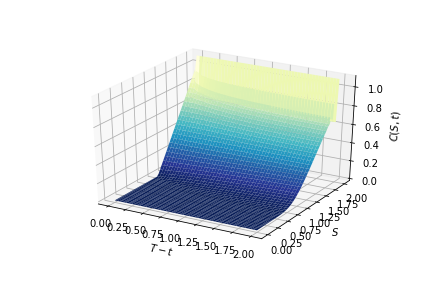
\includegraphics[width=\textwidth]{BSCNGrid.png}
    \caption{Output grid of Black-Scholes equation.}
  \end{minipage}
\end{figure}

\subsection{Alternating Direction Implicit Method}
The alternating direction implicit (ADI) method is one of the most common techniques to numerically solve two dimensional parabolic PDEs. ADI scheme give us advantages of the implicit finite difference method and computationally requires to solve only tridiagonal matrices. The scheme was first proposed by Peaceman and Rachford in 1955 for oil reservoir modelling \cite{peace}. Basically the methods to split the spatial dimensions and solve a two dimensional problem as two consecutive one dimensional problems. It is possible to use ADI in more than three dimensions which produces the same number of consecutive one dimensional problems \cite{DougADI}. In order to develop a more compact notation, we introduce the finite difference operator notation $\delta^2$.

\begin{equation}
\delta x^2 u^{n}_{i,j}  = \frac{u^{n}_{i+1,j} - 2u^{n}_{i,j} + u^{n}_{i-1,j}}{\Delta x^2}
\end{equation}

Explicit method in two space dimensions can be abbreviated as
\begin{equation}
\frac{u^{n+1}_{i,j} + u^{n}_{i,j}}{\Delta t} = \delta x^2 u^{n}_{i,j} + \delta y^2 u^{n}_{i,j}
\end{equation}
and implicit method in two space dimensions can be written as
\begin{equation}
\frac{u^{n+1}_{i,j} + u^{n}_{i,j}}{\Delta t} = \delta x^2 u^{n+1}_{i,j} + \delta y^2 u^{n+1}_{i,j} .
\end{equation}

Dividing each time step in half we introduce a temporary intermediate unknown $u^{n+1/2}_{i,j}$. Firstly, the two dimensional heat equation is approximating implicitly x and explicitly over y. The total work involved in one time step amounts to solving $ N_{steps} - 1$ tridiagonal systems \cite{morton}. 
\begin{equation}
\frac{u^{n+1/2}_{i,j} + u^{n}_{i,j}}{0.5 \Delta t} = \frac{\delta x^2 u^{n+1/2}_{i,j} }{\Delta x^2} + \frac{\delta y^2 u^{n}_{i,j}}{\Delta y^2}
\end{equation}
Rearranging the set of equations yields a tridiagonal system which is solved for the temporary intermediate unknown $u^{n+1/2}_{i,j}$.
\begin{equation}
- r_x u^{n+1/2}_{i+1,j} + (1 + 2r_x) u^{n+1/2}_{i,j}  - r_x u^{n+1/2}_{i,j}  = r_y u^{n}_{i,j+1} + (1 + 2r_y) u^{n}_{i,j} + r_y u^{n}_{i,j-1}
\end{equation}

\begin{figure}[!htb]
    \centering
        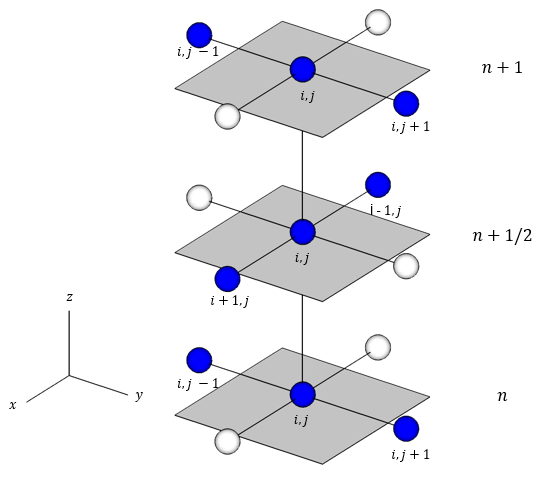
\includegraphics[scale=0.7]{ADI.png}
    \caption{Computational stencil of alternating direction implicit method}
\end{figure}

Next step of the grid $u^{n+1}_{i,j}$ is calculated by approximating explicitly x and implicitly over y.
\begin{equation}
\frac{u^{n+1}_{i,j} + u^{n+1/2}_{i,j}}{0.5 \Delta t} = \frac{\delta x^2 u^{n+1/2}_{i,j} }{\Delta x^2} + \frac{\delta y^2 u^{n+1}_{i,j}}{\Delta y^2}
\end{equation}

\begin{figure}[!htb]
    \centering
        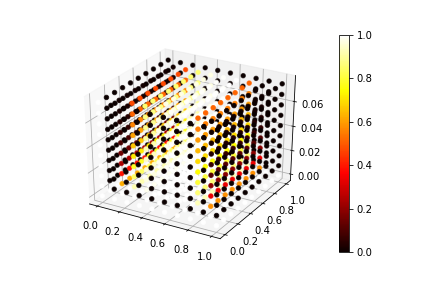
\includegraphics[scale=0.6]{ADIHeat.png}
    \caption{Solution of two dimensional heat equation using ADI.}
\end{figure}


Rearranging the set of equations yields a tridiagonal system which can be solved using Gaussian elimination, cyclic reduction or Thomas algorithm.
\begin{equation}
-r_y u^{n+1}_{i,j+1} + (1 + 2r_y) u^{n+1}_{i,j} - r_y u^{n+1}_{i,j-1} = r_x * u^{n+1/2}_{i+1,j} + (1 + 2r_x) u^{n+1/2}_{i,j} + r_x u^{n+1/2}_{i,j}
\end{equation}

$$
\begin{bmatrix}  
\theta & \lambda & 0 & . & . & 0 \\ 
\omega & \theta & \lambda & 0 & ... & . \\ 
0 & \omega & \theta & \lambda & 0 & . \\ 
. & . & .  & . & . & . \\ 
. & . & .  & . & . & . \\ 
. & . & .  & . & . & \lambda \\ 
0 & 0 & 0 & 0 & \omega & \theta \\ 
\end{bmatrix}  \begin{bmatrix} 
u_{1}^{n + 1} \\ 
u_{2}^{n + 1} \\ 
u_{3}^{n + 1} \\ 
.\\ 
.\\ 
.\\ 
u_{j - 1}^{n + 1}\\ 
\end{bmatrix}= \begin{bmatrix}
\alpha u_{0}^{n} \\ 
0 \\ 
0 \\ 
.\\ 
.\\ 
.\\ 
\gamma u_{j}^{n} \\ 
\end{bmatrix}  + \begin{bmatrix}  
\beta & \gamma & 0 & . & . & 0 \\ 
\alpha & \beta & \gamma & 0 & ... & . \\ 
0 & \alpha & \beta & \gamma & 0 & . \\ 
. & . & .  & . & . & . \\ 
. & . & .  & . & . & . \\ 
. & . & .  & . & . & \gamma \\ 
0 & 0 & 0 & 0 & \alpha & \beta \\ 
\end{bmatrix} \begin{bmatrix}  
u_{1}^{n} \\ 
u_{2}^{n} \\ 
u_{3}^{n} \\ 
.\\ 
.\\ 
.\\ 
u_{j - 1}^{n} \\ 
\end{bmatrix}
$$


\chapter{Optimizing Solvers}

Attempting to progress in solving complex problems using numerical methods is impossible without applying optimizations. However, nowadays the problem is not to solve a given problem but rather solve it in a given computing environment while exploiting the resources in an optimal way. Thus, it is necessary to investigate methods that allow for efficient implementations. The aim of this section is to introduce practical optimization techniques that can be easily implemented on a regular trading floor. Main optimization techniques that will be tested are parallelizing tridiagonal solvers, Visual Studio optimization switches, compilers and solution platforms.

\section{Solution Platforms}
The CPU accesses data from RAM using the register that stores memory addresses. 32 bit and 64 bit refers to the amount of data the system can access. so a 32-bit system can address a maximum of 4 GB (4,294,967,296 bytes) of RAM where a 64-bit register can theoretically reference 18,446,744,073,709,551,616 bytes, or 17,179,869,184 GB (16 exabytes) of memory. Since 32 bit does not have access to more than 4 GB, if the system has more than 4 GB of RAM, it will be inaccesible by the CPU, thus A 64 bit system will be needed. The memory increase of 64 bit systems means it is capable of very fast processing of numerical quantities. One disadvantage of the 64 bit systems is more requirement of memory because addresses are 64 bits (8 bytes) wide instead of 32 bits (4 bytes) wide. Due to the increased size of pointers and data structures, 64-bit programs will occupy more memory than an 32-bit version.

\section{Compilers}
A good compiler should let us focus on the process of writing programs rather than struggling with the inadequacies of the compiler. It should compile the most recent language standards without complaint. We should feel confident in its ability to produce well-optimized code from even the most abstract codebase. Lastly, it should compile source code as quickly as possible.

Regardless of the implementation of the program, the performance can be different under varying compilers. 

Modern CPUs are highly pipelined, superscalar machines that execute instructions out-of-order, use speculative execution, prefetching, and other performance-enhancing techniques. This makes it difficult to predict exactly how well a sequence of instructions will execute on any given microarchitecture. Hardware engineers use highly sophisticated simulations to overcome these problems when designing new CPUs. Compilers have to use heuristics to decide how to target specific CPU microarchitectures and thus have to be tuned to produce good code. Furthermore, the tuning is workload-specific, i.e., a generally sub-par compiler may produce the best code for certain workloads, even though it generally produces poorer code on average.


\section{Visual Studio Optimization Switches}
Visual Studio Optimization Switches, also known as /O options controls various optimizations to be chosen according to the needs of the project. There are various switches for different goals such as minimizing the size of the code (/O1) but since the scope of this project is limited with speed optimizations. Speed optimization flags are /O2 and /Ox. /O2 is a combination of /Og, /Oi, /Ot, /Oy, /Ob2, /GF and /Gy flags. /Ox is a subset of /O2 without the  /GF and /Gy flags. These additional options applied by /O2 can cause pointers to strings or to functions to share a target address, which can affect debugging and strict language conformance  \cite{vsopt}. 

\begin{itemize}
\item /Og: Enables local and global optimizations (subexpression elimination), automatic-register allocation, and loop optimization \cite{og}. 
\item /Oi: Generates intrinsic functions for appropriate function calls. Compiler may not replace the function call with an intrinsic if it will result in better performance \cite{oi}.
\item /Ot: Favors optimizations for speed over optimizations for size by instructing the compiler to reduce many C and C++ constructs to functionally similar sequences of machine code. If /Ot is used, /Og must be specified to optimize the code \cite{ot}.
\item /Oy: Suppresses the creation of frame (base) pointers on the call stack for quicker function calls.  Frees one register for general usage \cite{oy}.
\item /Ob2: Controls inline expansion of functions. Under /O2 and /Ox, allows the compiler to expand any function including the ones  that are not explicitly marked for no inlining. Function-calling-overheads are saved thus inline functions run faster than the normal functions with a memory penalty \cite{ob}.
\item /GF:  Enables the compiler to create a single copy of identical strings in the program image and in memory during execution. This is an optimization called string pooling that can create smaller programs. Under this flag, strings are pooled as read-only, trying to modify strings throws an error \cite{gf}.
\item /Gy: Enables function-level linking. Allows the compiler to package individual functions in the form of packaged functions  (COMDATs) or order individual functions in a DLL or .exe file \cite{gy}.
\end{itemize}

/O2 and /Ox flags are tested for maximum speed against the /Od flag which disables all the optimizations.
 
\section{Tridiagonal Solvers}
Tridiagonal solvers are the most demanding part of the solvers. Hence, development and improvement of such solvers is of great interest \cite{terekhov} \cite{chavez} \cite{hofen} \cite{austin} concerned with this problem. 


Large tridiagonal systems of linear equations appear in many numerical analysis applications. In our work, they arise in 

Implementing Crank Nicolson and Alternating Direction Implicit methods requires to solve tridiagonal systems which is the most computationally intensive part of the program.  Therefore, choosing efficient tridiagonal solvers is crucial for the speed of the solver. In this experiment three different algorithms will be tested.

Thomas algorithm which takes $O(N)$ steps and cyclic reduction which takes $2log_2 N$ steps

The Thomas algorithm is avery efficient algorithm for solving tridiagonal systems of equations in serial [15].It is equivalent to Gaussian elimination without pivoting;
\cite{duffycpp}

In this book we are mainly interested in solving tridiagonal systems of equations that arisewhen we discretise PDEs and two-point boundary value problems. In particular, these systemsarise when we approximate partial derivatives in the space dimension by three-point divideddifferences. In most cases we can use the popular Thomas algorithm to solve the resultinglinear system, although the Double Sweep method performs better. In particular, the Thomasalgorithm is used in the Alternating Direction Implicit (ADI) method which is one of the pop-ular schemes in computational finance

\subsection{Thomas Algorithm}
Thomas Algorithm is the most commonly used method for solving tridiagonal system of equations. The method is used to solve a tridiagonal matrix system invented by Llewellyn Thomas \cite{thomas}. The algorithm is a simplified version of the gaussian elimination.

The system equations can be written as
$$
\begin{bmatrix}  
b_1 & c_1 & 0 & 0 & ... & 0 \\ 
a_2 & b_2 & c_2 & 0 & ... & 0 \\ 
0 & a_3 & b_3 & c_3 & 0 & 0 \\ 
. & . &  &  &  & . \\ 
. & . &  &  &  & . \\ 
. & . &  &  &  & c_{k-1} \\ 
0 & 0 & 0 & 0 & a_k & b_k \\ 
\end{bmatrix} \begin{bmatrix}  
f_1 \\ 
f_2 \\ 
f_3 \\ 
.\\ 
.\\ 
.\\ 
f_k \\ 
\end{bmatrix} = \begin{bmatrix} 
d_1 \\ 
d_2 \\ 
d_3 \\ 
.\\ 
.\\ 
.\\ 
d_k \\ 
\end{bmatrix}
$$

The method begins by forming coefficients \(c^{*}_i\) and \(d^{*}_i\) in place of \(a_i\), \(b_i\) and \(c_i\) as follows:
$$
c^{*}_i = \left\{
     \begin{array}{lr}
       \frac{c_1}{b_1} & ; i = 1\\
       \frac{c_i}{b_i - c^{*}_{i-1} a_i} & ; i = 2,3,...,k-1
     \end{array}
   \right.
$$
$$   
d^{*}_i = \left\{
     \begin{array}{lr}
       \frac{d_1}{b_1} & ; i = 1\\
       \frac{d_i-d^{*}_{i-1} a_i}{b_i - c^{*}_{i-1} a_i} & ; i = 2,3,...,k-1
     \end{array}
   \right.
   $$
With these new coefficients, the matrix equation can be rewritten as:
$$
\begin{bmatrix}  
1 & c^{*}_1 & 0 & 0 & ... & 0 \\ 
0 & 1 & c^{*}_2 & 0 & ... & 0 \\ 
0 & 0 & 1 & c^{*}_3 & 0 & 0 \\ 
. & . &  &  &  & . \\ 
. & . &  &  &  & . \\ 
. & . &  &  &  & c^{*}_{k-1} \\ 
0 & 0 & 0 & 0 & 0 & 1 \\ 
\end{bmatrix} \begin{bmatrix}  
f_1 \\ 
f_2 \\ 
f_3 \\ 
.\\ 
.\\ 
.\\ 
f_k \\ 
\end{bmatrix} = \begin{bmatrix} 
d^{*}_1 \\ 
d^{*}_2 \\ 
d^{*}_3 \\ 
.\\ 
.\\ 
.\\ 
d^{*}_k \\ 
\end{bmatrix}
$$
The algorithm for the solution of these equations is now straightforward and works 'in reverse':

\[ f_k = d^{*}_k, \qquad f_i = d^{*}_k - c^{*}_i x_{i+1}, \qquad i = k-1, k-2, ... ,2,1 \]

 \subsection{Intel Math Kernel Library}
Intel Math Kernel Library implements routines for solving systems of linear equations from the standard LAPACK library. Variety of atrix types are supported by the routines.  Specifically gtsv function is utilized from the package. Using Gaussian elimination with partial pivoting, gstv computes the solution to the system of linear equations with a tridiagonal coefficient matrix \cite{gtsv}.  

\subsection{Cyclic Reduction}\label{cyclic}
Cyclic reduction was proposed by R. W. Hockney in the 1960s for solving the resulting linear systems from the  discretization of the Poisson equation \cite{Hockney}. 

$$
\begin{bmatrix}  
1 & c^{*}_1 & 0 & 0 & ... & 0 \\ 
0 & 1 & c^{*}_2 & 0 & ... & 0 \\ 
0 & 0 & 1 & c^{*}_3 & 0 & 0 \\ 
. & . &  &  &  & . \\ 
. & . &  &  &  & . \\ 
. & . &  &  &  & c^{*}_{k-1} \\ 
0 & 0 & 0 & 0 & 0 & 1 \\ 
\end{bmatrix} \begin{bmatrix}  
f_1 \\ 
f_2 \\ 
f_3 \\ 
.\\ 
.\\ 
.\\ 
f_k \\ 
\end{bmatrix} = \begin{bmatrix} 
d^{*}_1 \\ 
d^{*}_2 \\ 
d^{*}_3 \\ 
.\\ 
.\\ 
.\\ 
d^{*}_k \\ 
\end{bmatrix}
$$

Let $a$, $b$, 

If we number equations succesively, then in cyclic reduction the odd-neighbor equations of an even equation are used to eliminate the off-diagonal entries in the even equation.In this step, a tridiagonal system of linear equations for the even equation is gener-ated. This reduced system has only about one-half as many equations as the originalsystem. Now the same procedure is applied recursively to the reduced system untilthere remains only one linear equation with one unknown. The solution of successivereduced systems can be computed to finally yield the solution of the original system.


\begin{figure}[!htb]
    \centering
        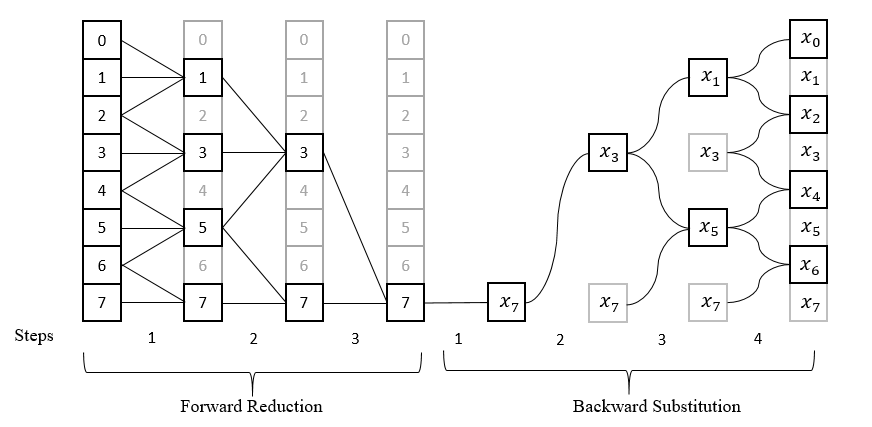
\includegraphics[scale=0.6]{cyclic.png}
    \caption{Cyclic reduction for an eight equation system.}
\end{figure}

If serially computed, Thomas algorithm performs $8n$ operations while CR performs $17n$ operations. On the other hand,if parallel computing is used with $n$ cores, CR requires $2 log_2 n − 1$ steps  while  the  Thomas algorithm requires $2n$ steps \cite{gputri}. CPU parallelism will be used to test cyclic reduction.


\section{Open Multi-Processing}
Traditionally, programs are serially computed on a single processor. On the other hand, parallel computation is used to break our code execution in pieces so that it utilizes parallelism. Multithreading uses the CPUs cores to run calculations concurrently in each core. The concurrent programs are called a thread. If the code is executed on parallel processors, one of the biggest problem is the processors generally require results that have been calculated on other processors. The main issue in this case is that processors clocks are not synchronized and execute the code at minimally different speeds.

\begin{figure}[!htb]
    \centering
        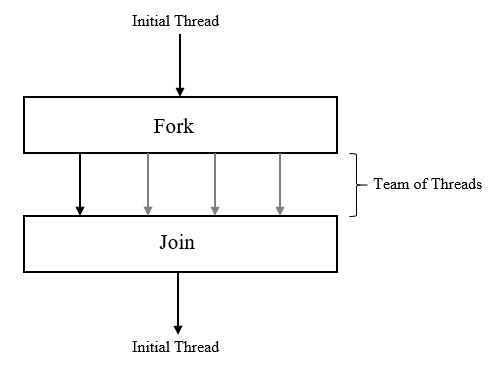
\includegraphics[scale=0.7]{openmp.png}
    \caption{The fork-join programming model.}
\end{figure}

In order to solve this problem, a group of major computer hardware and software vendors and major parallel computing user facilities joined forces to form The Open Multi-Processing Architecture Review Board (The OpenMP ARB)\cite{openmpfaq}. Open Multi-Processing (OpenMP) is an implementation of multithreading for C, C++ and Fortran and it was introduced to public in 1997. OpenMP is aiming to standardize high level parallelism that is performant, productive and portable.

 OpenMP approach to multithreading is the fork-join programming model. Firstly, the program start as a single thread of execution called the initial thread. The fork stage begins when the program encounters an OpenMP parallel construct. Parallel execution takes place and multiple threads are created in the parallel region. The initial thread becomes the master and collaborates with the newly created threads to execute the code dynamically. Finally, at the join stage all threads are synchronized, threads are terminated except the original thread \cite{openmp}.


Algorithms like cyclic reduction \ref{cyclic} uses nested loops to calculate the solution. Therefore nested parallelism is needed to build efficient programs. Nesting the parallel constructs results in nested parallelism. Each thread that encounters the next parallel region creates a new parallel region at runtime \cite{openmpnext}.

\begin{figure}[!htb]
    \centering
        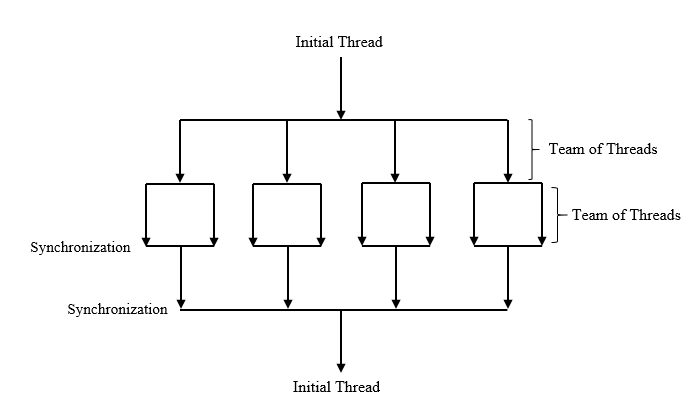
\includegraphics[scale=0.7]{openmpnested.png}
    \caption{4 threads create 2 threads, nested parallelism.}
\end{figure}

In order to specify and control the paralelization procedure, OpenMP uses compiler directives, runtime functions, and  envi­ronment variables. OpenMP enables developers to just give a high-level specification of the parallelism by indicating the regions to be executed in parallel using compiler directives, runtime library routines, and environment variables. The details of the parallelism is up to the compiler which makes OpenMP comparatively easy to use. 

\section{Timing the Code}
Measuring execution time intervals accurately is an important aspect to compare the efficiency and speed of different environments and implementations.

\subsection{Windows Application Programming Interface}
Windows Application Programming Interface (API) is the lowest level of interaction between applications and the windows operating system. Thus every program is built upon  the API. Mostly, the interaction is hidden, the runtime and support libraries manage it in the background \cite{windows}. The APIs can be used in the C++ environment. Runtime can be calculated by "QueryPerformanceCounter" or "QueryPerformanceFrequency"  functions. Respectively, the functions retrieve a high resolution time stamp and the frequency of the performance counter. 

\subsection{Chrono Library}
Using the Windows API for just timing the code is slightly excessive given the amount of work it takes. Luckily, Chrono library was introduced part of the C++11’s standard library.  Timers and clocks might differ on distinct systems, thus Chrono library is designed to work effortlessly with date and time. The "high resolution clock" provides the smallest possible tick period and with the “now” method, returns a value corresponding to the call’s point in time.  Once the start and end time of the code is recorded ,  the duration::count method is used to get the elapsed time.


\section{Comparison of Optimizations}
This section documents the performance of attempted optimizations. Experiments  are  conducted  at  W307 computer laboratory, Queen Mary University of London.  Each computer has Windows 10 Enterprise 64 bit, 16 GB of RAM, Intel Core i7-6700 CPU with 4 cores clocked at 3.40 GHz.  The source code is written in C++ and compiled with Microsoft Visual Studio Enterprise 2017, Version 15.3.3 in the release mode. External tools  utilized  in  the  tests  include Intel Compiler, version 18.0.3 and Intel Math Kernel  Library. 

Numerical analysis and computer simulations is undertaken to put theory and observation together to gain insight into the workings of numerical solutions of partial differential equations. First step was solving the base cases \ref{bsAnal}, \ref{HeatBase}, \ref{HeatTwoBase} by hand and Excel. Following the simple implementations, the solvers are ported to C++ to measure and optimize the performance.
Different solution platforms, compilers, optimization flags and tridiagonal solvers will be tested against each other.
 
\subsection{Optimal Grid Size}
Previously defined analytical solutions \ref{bsAnal}, \ref{heatAnal}, \ref{heat2Anal} are utilised to calculate errors for the solutions using different grid sizes, the grid with the lowest error is used for further tests. Figure X and X demonstrates the error compared to the grid sizes. The optimal grid size for heat equation and Black-Scholes equation is 50 by 50.


 
\begin{figure}[!htb]
  \begin{minipage}[b]{0.5\textwidth}
    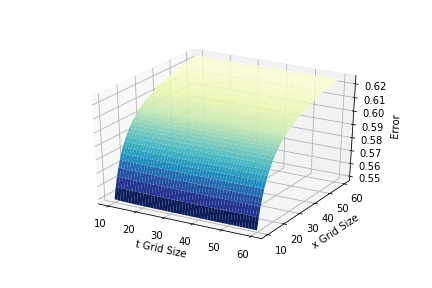
\includegraphics[width=\textwidth]{HeatExplicitGridError.png}
    \caption{Error of grid sizes.}
  \end{minipage}
  \begin{minipage}[b]{0.5\textwidth}
    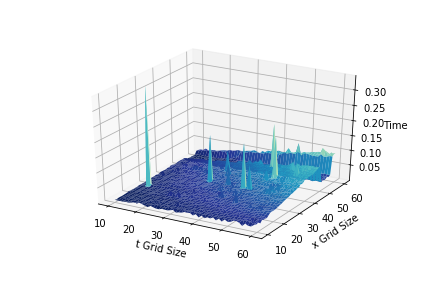
\includegraphics[width=\textwidth]{HeatExplicitGridTimer.png}
    \caption{Timing grid sizes.}
  \end{minipage}
\end{figure}


\begin{figure}[!htb]
  \begin{minipage}[b]{0.5\textwidth}
    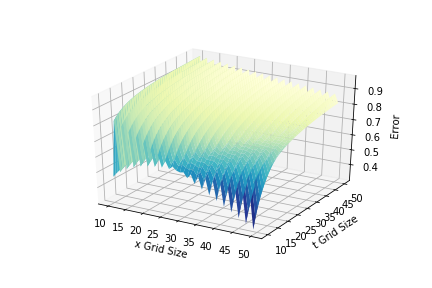
\includegraphics[width=\textwidth]{BSExplicitGridError.png}
    \caption{Error of grid sizes.}
  \end{minipage}
  \begin{minipage}[b]{0.5\textwidth}
    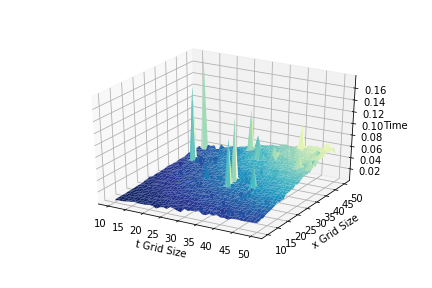
\includegraphics[width=\textwidth]{BSExplicitGridTimer.png}
    \caption{Timing grid sizes.}
  \end{minipage}
\end{figure}

\subsection{Base Case}
Timing the base case for thomas algorithm, intel solver and cyclic reduction. The timings are mean of 1000 trials and each trial adds a random number $ 0 < \epsilon < 10^-7 $ to the step size to avoid compiler optimizations.

\begin{table}[h!]
\centering
 \begin{tabular}{||c c c||} 
 \hline
 Environment & Explicit Method & Crank Nicolson\\ [0.5ex] 
 \hline\hline\hline
 Visual Studio Compiler x86 & 0.02496743 & 0.02590181 \\ 
 Visual Studio Compiler x64 & 0.02105383 & 0.02216256 \\
 Intel Compiler x86 & 0.02563324 & 0.02633357 \\
 Intel Compiler x64 & 0.02210323 & 0.02298945\\ [1ex] 
 \hline
 \end{tabular}
 \caption{Solving Black-Scholes with Thomas Algorithm base case.}
\end{table}

\begin{table}[h!]
\centering
 \begin{tabular}{||c c c||} 
 \hline
 Environment & Explicit Method & Crank Nicolson\\ [0.5ex] 
 \hline\hline\hline
 Visual Studio Compiler x86 &  \\ 
 Visual Studio Compiler x64 & \\
 Intel Compiler x86 & \\
 Intel Compiler x64 & 0.02171834 & 0.02286124\\ [1ex] 
 \hline
 \end{tabular}
 \caption{Solving Black-Scholes with Intel Solver base case.}
\end{table}

\begin{table}[htp!]
\centering
 \begin{tabular}{||c c c c||} 
 \hline
 Testing & Explicit Method & Crank Nicolson & ADI\\ [0.5ex] 
 \hline\hline\hline
 Visual Studio Compiler x86 & 0.02502006 & 0.02536817 & 0.07766176 \\ 
 Visual Studio Compiler x64 & 0.02185875 & 0.02211793 & 0.06512516 \\
 Intel Compiler x86 & 0.02685609 & 0.02694334 & 0.08277156\\
 Intel Compiler x64 & 0.0225934 & 0.0226115 & 0.06614703\\[1ex] 
 \hline
 \end{tabular}
 \caption{Solving heat equation with Thomas Algorithm base case.}
\end{table}
 
 
\begin{table}[htp!]
\centering
 \begin{tabular}{||c c c c||} 
 \hline
 Testing & Explicit Method & Crank Nicolson & ADI\\ [0.5ex] 
 \hline\hline\hline
 Visual Studio Compiler x86 \\ 
 Visual Studio Compiler x64 &  \\
 Intel Compiler x86 & \\
 Intel Compiler x64 & 0.02239165 & 0.02195975 & 0.06337759\\[1ex] 
 \hline
 \end{tabular}
 \caption{Solving heat equation with Intel Solver base case.}
\end{table}
 

\subsection{Visual Studio Optimizations} 
 The optimization switch for enabling most speed optimizations /Ox will be utilized in this section. 
\begin{table}[h!]
\centering
 \begin{tabular}{||c c c||} 
 \hline
 Environment & Explicit Method & Crank Nicolson\\ [0.5ex] 
 \hline\hline\hline
 Visual Studio Compiler x86 & \\ 
 Visual Studio Compiler x64 & \\
 Intel Compiler x86 & \\
 Intel Compiler x64 & \\ [1ex] 
 \hline
 \end{tabular}
 \caption{Solving Black-Scholes with Thomas Algorithm using Visual Studio optimizations.}
\end{table}

\begin{table}[h!]
\centering
 \begin{tabular}{||c c c||} 
 \hline
 Environment & Explicit Method & Crank Nicolson\\ [0.5ex] 
 \hline\hline\hline
 Visual Studio Compiler x86 & \\ 
 Visual Studio Compiler x64 & \\
 Intel Compiler x86 & \\
 Intel Compiler x64 & \\ [1ex] 
 \hline
 \end{tabular}
 \caption{Solving Black-Scholes with Intel Solver using Visual Studio optimizations.}
\end{table}

\begin{table}[htp!]
\centering
 \begin{tabular}{||c c c c||} 
 \hline
 Testing & Explicit Method & Crank Nicolson & ADI\\ [0.5ex] 
 \hline\hline\hline
 Visual Studio Compiler x86 \\ 
 Visual Studio Compiler x64 & \\
 Intel Compiler x86 & \\
 Intel Compiler x64 & \\[1ex] 
 \hline
 \end{tabular}
 \caption{Solving heat equation with Thomas Algorithm using Visual Studio optimizations.}
\end{table}
 
 
\begin{table}[htp!]
\centering
 \begin{tabular}{||c c c c||} 
 \hline
 Testing & Explicit Method & Crank Nicolson & ADI\\ [0.5ex] 
 \hline\hline\hline
 Visual Studio Compiler x86 \\ 
 Visual Studio Compiler x64 & \\
 Intel Compiler x86 & \\
 Intel Compiler x64 & \\[1ex] 
 \hline
 \end{tabular}
 \caption{Solving heat equation with Intel Solver using Visual Studio optimizations.}
\end{table}

\subsection{Cyclic Reduction with OpenMP} 
 
\begin{table}[h!]
\centering
 \begin{tabular}{||c c c||} 
 \hline
 Environment & Cyclic Reduction\\ [0.5ex] 
 \hline\hline\hline
 Visual Studio Compiler x86 & 0\\ 
 Visual Studio Compiler x64 & 0 \\
 Intel Compiler x86 & 0\\
 Intel Compiler x64 &0 \\ [1ex] 
 \hline
 \end{tabular}
 \caption{Solving Black-Scholes with cyclic reduction.}
\end{table}

\begin{table}[h!]
\centering
 \begin{tabular}{||c c c||} 
 \hline
 Environment & Cyclic Reduction\\ [0.5ex] 
 \hline\hline\hline
 Visual Studio Compiler x86 & 0\\ 
 Visual Studio Compiler x64 & 0 \\
 Intel Compiler x86 & 0\\
 Intel Compiler x64 &0 \\ [1ex] 
 \hline
 \end{tabular}
 \caption{Solving heat equation with cyclic reduction.}
\end{table}

\chapter{Conclusion}
A Critique of the Crank Nicolson Scheme Strengths and Weaknesses for FinancialInstrument Pricing + rannacher 
AVX and Intrinsics CPUs are pipelining and use of SSE/SIMD kusswurm registers with Advanced Vector Extensions(AVX 512)GPGPU In the case of General Purpose GPUs, CUDA or Open Computing Language(OpenCL) can be utilized but can be challenging because of the requirement of delicate memory management. \cite{fpga},  cloud functions \cite{cloudfunc}.
change black scholes to a different pricing pde like interest rate derivatives The HJM model \cite{kohl}
Results concludela

\appendix
\chapter{Usage of chrono class}
Should code example be in appendix or stay here?
\begin{verbatim}
auto start = std::chrono::high_resolution_clock::now();
    Portion of code to be timed
auto finish = std::chrono::high_resolution_clock::now();
std::chrono::duration<double> elapsed = finish - start;
std::cout << "Elapsed time: " << elapsed.count() << " s\n";
\end{verbatim}

\chapter{Implementation of the {\tt PDE} class}
Parabolic partial differential equation can be denoted as
$$ \frac{\partial u}{\partial t} = a(t,x) \frac{\partial^2 u}{\partial x^2} + b(t,x) \frac{\partial u}{\partial x} + c(t,x) u(t,x) + d(t,x) $$

$a(t,x)$ denotes diffusion coefficient,  $b(t,x)$ convection coefficient, $c(t,x)$ reaction coefficient, $d(t,x)$ source coefficient
analytic solution, initial conditions boundary conditions
\chapter{Implementation of the {\tt FiniteDifferenceMethod} class}

\begin{verbatim}
void stepSize();
void initialConditions();
void boundaryConditions();
void innerDomain();
void timeMarch();
\end{verbatim}



\bibliographystyle{plain}
\bibliography{ThesisDraft}

\end{document}
